\documentclass{beamer}
\usetheme{Warsaw}
\setbeamertemplate{footline}[frame number]

\usepackage[utf8]{inputenc}
\usepackage{fancybox}
\usepackage{multimedia} 
\usepackage{subfig}
\usepackage{amsmath}
\usepackage{hyperref}
\usepackage[all]{xy}
\begin{document}


\title[Angewandte Mathematik] % (optional, only for long titles)
{Angewandte Mathematik
\\
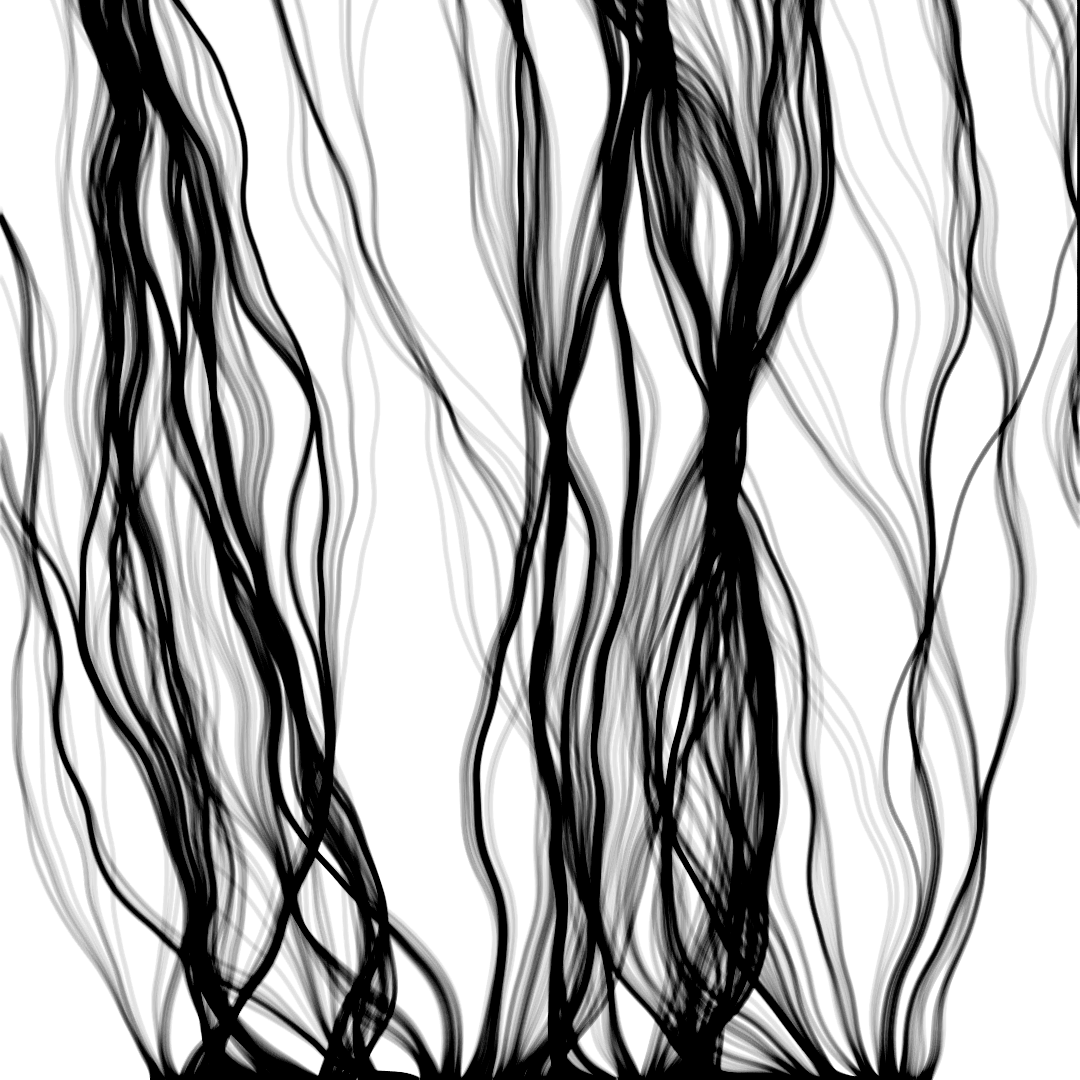
\includegraphics[scale=0.15]{images/cover}
}
\subtitle{}
\author[Dr. Johannes Riesterer] % (optional, for multiple authors)
{Dr.  rer. nat. Johannes Riesterer}

\date[KPT 2004] % (optional)
{}

\subject{Angewandte Mathematik}

\frame{\titlepage}

\begin{frame}
    \frametitle{Angewandte Mathematik}
\framesubtitle{Einleitung Lean}
    \begin{block}{Was ist Lean?}
        \begin{itemize}
            \item Ein interaktiver Theorembeweiser und Programmiersprache.
            \item Wird verwendet, um mathematische Aussagen formal zu beweisen und zu verifizieren.
            \item Besitzt eine aktive und wachsende Community, insbesondere in der formalen Mathematik.
        \end{itemize}
    \end{block}

\begin{block}{Curry Howard Isomorphismus}
     Basiert auf dem Curry-Howard-Isomorphismus.
     Der Curry-Howard-Isomorphismus besagt, dass logische Aussagen als Typen und Beweise als Programme betrachtet werden können. Mit anderen Worten:
    \begin{itemize}
        \item Logische Aussagen $\leftrightarrow$ Typen
    
        \item Beweise von Aussagen $\leftrightarrow$  Programme, die zu diesen Typen gehören
    \end{itemize}
    \end{block}

 \end{frame}


% Folie 1: Einleitung
\begin{frame}{Einleitung}
    \textbf{Curry-Howard-Isomorphismus}: Eine Beziehung zwischen Logik und Typentheorie. \\
    \vspace{0.5cm}
    Logische Aussagen entsprechen Typen, Beweise entsprechen Programmen. \\
    \vspace{0.5cm}
    \begin{itemize}
        \item \textbf{Konjunktion (\(\wedge\))} als Produkt-Typ
        \item \textbf{Disjunktion (\(\vee\))} als Summen-Typ
        \item \textbf{Implikation (\(\Rightarrow\))} als Funktionstyp
        \item \textbf{Allquantor (\(\forall\))} als Produkttyp
        \item \textbf{Existenzquantor (\(\exists\))} als Summentyp
    \end{itemize}
\end{frame}

% Folie 2: Produkttyp (Konjunktion)
\begin{frame}{Konjunktion (\(\wedge\)) und Produkttyp}
    \begin{block}{Definition}
        Die Konjunktion \( A \wedge B \) entspricht einem Produkttyp \( A \times B \). \\
        Ein Beweis für \( A \wedge B \) ist ein Paar \((a, b)\), wobei \( a \) ein Beweis für \( A \) und \( b \) ein Beweis für \( B \) ist.
    \end{block}

    \begin{block}{NOTATION}
        \[
        A \wedge B \quad \Rightarrow \quad A \times B
        \]
    \end{block}
    
    \textbf{Beispiel:} \\
    Angenommen \( A = \text{"gerade Zahl"} \) und \( B = \text{"größer als 2"} \). \\
    Ein Beweis von \( A \wedge B \) ist ein Paar aus einer geraden Zahl \( x \) und der Eigenschaft \( x > 2 \).
\end{frame}

% Folie 3: Summentyp (Disjunktion)
\begin{frame}{Disjunktion (\(\vee\)) und Summentyp}
    \begin{block}{Definition}
        Die Disjunktion \( A \vee B \) entspricht einem Summentyp \( A + B \). \\
        Ein Beweis für \( A \vee B \) ist entweder ein Beweis für \( A \) oder ein Beweis für \( B \).
    \end{block}

    \begin{block}{NOTATION}
        \[
        A \vee B \quad \Rightarrow \quad A + B
        \]
    \end{block}

    \textbf{Beispiel:} \\
    Angenommen \( A = \text{"gerade Zahl"} \) und \( B = \text{"ungerade Zahl"} \). \\
    Ein Beweis für \( A \vee B \) ist entweder eine gerade oder eine ungerade Zahl.
\end{frame}

% Folie 4: Funktionstyp (Implikation)
\begin{frame}{Implikation (\(\Rightarrow\)) und Funktionstyp}
    \begin{block}{Definition}
        Die Implikation \( A \Rightarrow B \) entspricht einem Funktionstyp \( A \to B \). \\
        Ein Beweis für \( A \Rightarrow B \) ist eine Funktion, die aus einem Beweis für \( A \) einen Beweis für \( B \) konstruiert.
    \end{block}

    \begin{block}{NOTATION}
        \[
        A \Rightarrow B \quad \Rightarrow \quad A \to B
        \]
    \end{block}

    \textbf{Beispiel:} \\
    Angenommen \( A = \text{"gerade Zahl"} \) und \( B = \text{"die Verdopplung ist auch gerade"} \). \\
    Ein Beweis für \( A \Rightarrow B \) ist eine Funktion, die jede gerade Zahl \( n \) auf die Aussage abbildet, dass \( 2n \) auch gerade ist.
\end{frame}

% Folie 5: Abhängiger Typ - Allquantor (\(\forall\))
\begin{frame}{Allquantor (\(\forall\)) als Produkttyp}
    \begin{block}{Definition}
        Der Allquantor \( \forall x \in A \, . \, P(x) \) entspricht einem Produkttyp \( \prod_{x : A} P(x) \). \\
        Ein Beweis für \( \forall x \in A \, . \, P(x) \) ist eine Funktion, die jedem \( x \in A \) einen Beweis für \( P(x) \) zuordnet.
    \end{block}

    \begin{block}{NOTATION}
        \[
        \forall x \in A \, . \, P(x) \quad \Rightarrow \quad \prod_{x : A} P(x)
        \]
    \end{block}

    \textbf{Beispiel:} \\
    "Für jede natürliche Zahl \( n \) ist \( n \geq 0 \)":
    \[
    \forall n \in \mathbb{N} \, . \, n \geq 0 \quad \Rightarrow \quad \prod_{n : \mathbb{N}} (n \geq 0)
    \]
\end{frame}

% Folie 6: Abhängiger Typ - Existenzquantor (\(\exists\))
\begin{frame}{Existenzquantor (\(\exists\)) als Summentyp}
    \begin{block}{Definition}
        Der Existenzquantor \( \exists x \in A \, . \, P(x) \) entspricht einem Summentyp \( \sum_{x : A} P(x) \). \\
        Ein Beweis für \( \exists x \in A \, . \, P(x) \) ist ein Paar \((x, \text{Beweis für } P(x))\), wobei \( x \in A \) und \( P(x) \) gilt.
    \end{block}

    \begin{block}{NOTATION}
        \[
        \exists x \in A \, . \, P(x) \quad \Rightarrow \quad \sum_{x : A} P(x)
        \]
    \end{block}

    \textbf{Beispiel:} \\
    "Es gibt eine natürliche Zahl \( n \), die größer als 10 ist":
    \[
    \exists n \in \mathbb{N} \, . \, n > 10 \quad \Rightarrow \quad \sum_{n : \mathbb{N}} (n > 10)
    \]
\end{frame}


\begin{frame}
    \frametitle{Angewandte Mathematik}
\framesubtitle{Einleitung Lean}
    \begin{block}{Lean Installation}
        \begin{itemize}
            \item TODO
        \end{itemize}
    \end{block}
 \end{frame}


\end{document}

